\documentclass[parskip=half]{scrartcl}
	
\usepackage[english]{babel}
\usepackage[latin1]{inputenc}
\usepackage{enumerate} % til \begin{enumerate}[(i)]
\usepackage{enumitem} % til at styre lister globalt
\usepackage{latexsym} % symboler
\usepackage{amsthm} % til thm osv
\usepackage{amssymb} % flere symbloer
\usepackage{bm} % bold math symbols
\usepackage{amsmath} % til pmatrix
\usepackage[hyphens]{url} %til \url med bindestreger
%\PassOptionsToPackage{hyphens}{url}\usepackage{hyperref}
\usepackage[pdftex]{graphicx}	
\usepackage{scrlayer-scrpage} % page setup

\usepackage[section]{placeins} 

\usepackage{framed}
\usepackage[cache=false]{minted} % for source code
%\usepackage{xcolor}
%set page header
\chead{FYS-STK4155 --- project 3}


% List will number things using (a), (b), ...
\setenumerate[1]{label={(\alph*)}} % Global setting

% Title setup
\title{Report for Project 3}
\date{\today}
\author{Jon Audun, Mikael Ravndal and Adam P W S{\o}rensen}

\newcommand{\setof}[2]{\left\{ #1 \; \middle\vert \; #2 \right\}}

\DeclareMathOperator{\cspan}{\overline{span}}

% Theorem opsætning
\newtheorem{theorem}{Theorem}[section]
\newtheorem*{theorem*}{Theorem}
\newtheorem{lemma}[theorem]{Lemma}
\newtheorem{corollary}[theorem]{Corollary}
\newtheorem{proposition}[theorem]{Proposition}
\newtheorem{example}[theorem]{Example}
\newtheorem{conjecture}[theorem]{Conjecture}
\theoremstyle{definition}
\newtheorem{definition}[theorem]{Definition}
\newtheorem{assumption}[theorem]{Standing Assumption}
\newtheorem*{assumption*}{Standing Assumption}
\theoremstyle{remark}
\newtheorem{remark}[theorem]{Remark}
\newtheorem{notation}[theorem]{Notation}

%%%%%%%%%%%%
% notation short cuts
\newcommand{\vect}[1]{{\bm{#1}}}
\newcommand{\funcname}[1]{{\color{blue}{\texttt{#1}}}}
\newcommand{\varname}[1]{\texttt{#1}}
%%%%%%%%%%%%
% bb letters
\newcommand{\C}{\mathbb{C}}
\newcommand{\E}{\mathbb{E}}
\newcommand{\N}{\mathbb{N}}
\newcommand{\Q}{\mathbb{Q}}
\newcommand{\R}{\mathbb{R}}
\newcommand{\Z}{\mathbb{Z}}
% cal letters
\newcommand{\A}{\mathcal{A}}
\newcommand{\B}{\mathcal{B}}
\newcommand{\D}{\mathcal{D}}
\newcommand{\cL}{\mathcal{L}}
\newcommand{\M}{\mathcal{M}}
\newcommand{\cZ}{\mathcal{Z}}
% frak letters
\newcommand{\fA}{\mathfrak{A}}


%%%%%%%%%%%%%%
\begin{document}
%%%%%%%%%%%%%%

\maketitle

\begin{abstract}
In this project we work on a classification problem for cooking data coming from an old kaggle competition.
We investigate four single classifier methods, logistic regression, support vector machines, random forests and multilayer perceptrons (neural networks). 
We used cross validation to tune the models.
The best single classifier model was support vector machines which had a predicted accuracy of $\approx 0.78$. 
Using voting classifiers we combined our models to get a predicted accuracy of $\approx 0.80$. 

We made a late submission to kaggle and got an accuracy of $\approx 0.80$, which was about $0.02$ worse than the winning submission. 
\end{abstract}


\section{Introduction}

In this project we explore a delicious classification problem: 
Given a list of ingredients, can you predict what cuisine the final dish will be?
There are certainly cases where this is easy. 
If you meet your friend at the store and they have burritos, guacamole, salad, and beef in their basket, you can feel confident they are having Mexican food. 
But what if they have flour, yeast, and milk? 
They are probably baking, but are they making a French baguette or an Indian naan bread?   

We aim to investigate the performance of four different
machine learning techniques when applied to this problem: 
logistic regression, support vector machines, random forests and neural
networks. Will 
some of the methods outperform the others by far? Or will some of the 
methods perhaps be useless on this dataset?
We choose to use cross-validation as our main tool in trying to answer 
these questioins.

Our dataset comes from an old kaggle competition. 
It consists of 39,774 recipes which spans over 20 different cuisines.
The following plot shows their distribution among the 20 cuisines:

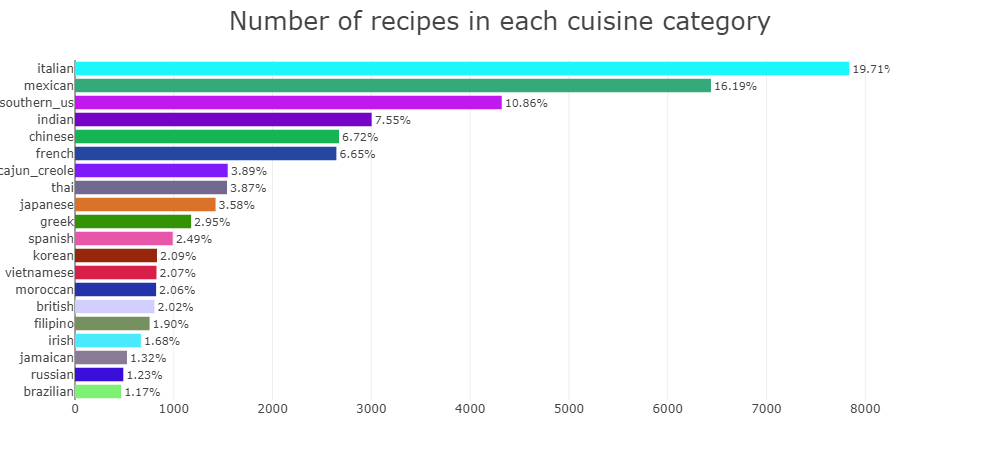
\includegraphics[scale=.42]{images/cuisine_number}
We can tell from the plot that around 36\% of the data is labeled as either italian or mexican cuisine. So we should be prepared on that this uneven distribution of the recipes will affect how our predictors will do.

It is also interesting to look at what the most common ingredients are:

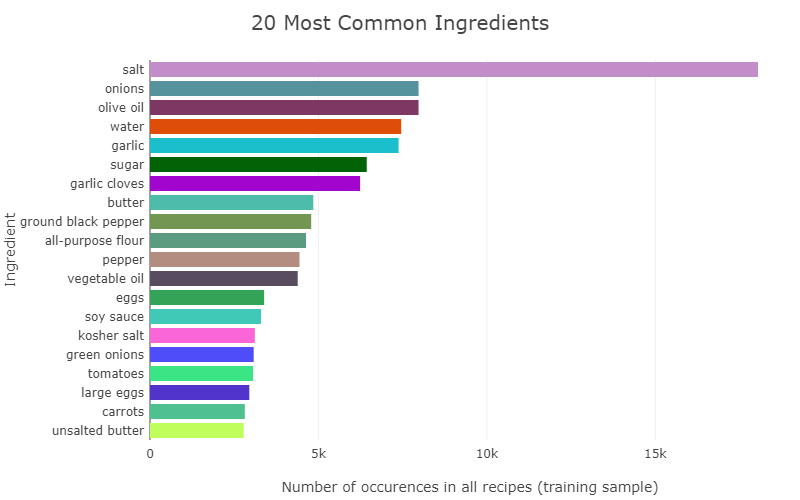
\includegraphics[scale=.55]{images/common_ing}
Salt is the most common ingredient by far. It is so common, that we can expect it to not be as good of a classifier as it probably won't be particular for a certain cuisine.
The other ingredients are more evenly spread out, which is expected.
More metadata can be found in the notebook "Descriptive analysis.ipynb"

The paper is organized as follows: 
\begin{itemize}
    \item
        \textbf{Methods}: 
        We start out by establishing how the four machine learning 
        teqhniques actually work and explain how we preprocess and
        format our dataset.
    \item
        \textbf{Model selection and verification}:
        In this section we start to present our own work.
        We report how we tuned our models by searching
        over grids of parameters, and how
        we finally used these results to create a voting classifier.
    \item
        \textbf{Results and discussion}:
        We discuss our final results and some thoughts on how we possibly
        could have made some further improvement.
    \item
        \textbf{Conclusion}:
        We close off by summarizing our findings.
    \item
        \textbf{Appendices}:
        Attached is prints of the jupyter notebooks. 
\end{itemize}

\begin{framed}
All the code we have implemented can be found at \url{https://github.com/jonabaa/Project3/tree/master/code}. The files that this report reffers to
are:
    \begin{itemize}
        \item
            testing.ipynb - this notebook 
            contains all the testing of our methods
        \item
            functions.py - this file contains functions we implemented in
            order to test our methods
        \item
            Kaggle submission script.ipynb - this file contains the script
            for submitting our model of choice to the kaggle.com contest
        \item
            Descriptive analysis.ipynb - this notebook contains some 
            descriptive analysis of our dataset, just to get a feel of
            what we are working with
    \end{itemize}
\end{framed}

\section{Methods} \label{sec:methods}

First we need to establish some notation. In the following we assume
that we are given $N \in \N$ samples consisting of $p \in \N$ features
and one target. Further we let $K \in \N$ be the number of
classes in our classification problem. We then denote by $x_{i,j}$ the
$j$-th feature of the $i$-th sample and by $t_i \in \{1,2, \dots, K\}$
the target of the $i$-th sample. 

\subsection{Reading in the data}
The raw data lives in a .json file, which we load using Pandas.
Each recipe has a cuisine and a list of ingredients. 
The first thing we do is to join all the ingredients into one string, and then we use scikit learns  \funcname{CountVectorizer} on the corpus of all recipes to get a matrix representation of the data. 
The \funcname{CountVectorizer} works by making each individual word in the whole corpus a feature.
Each recipe is then a vector in $\R^p$, with the $k$'th entry equal to the number of times the $k$'th feature (ingredient) appears in the recipe, usually this will be 0 or 1. 
This means that a recipe that calls for tomato sauce will have the features tomato and sauce set to 1, even if it does not use a tomato.

Before using the \funcname{CountVectorizer} we clean up the data a little bit, namely we replace hyphens with spaces, to make sure e.g. \emph{low-fat} and \emph{low fat} are treated the same, and we drop all numbers and special characters. 
The latter because the recipes are not all formatted in the same way, with some including amounts.
When using \funcname{CountVectorizer} we set the parameter \varname{min\_df} to 3.
This means we only include features that appear at least 3 times in all lists of ingredients.
We do this to make all our cross validation work meaningful. 
A feature that only appears once is useless for prediction, because it will either be contained only in the
training data or only in the test data. 
We also excluded features that only appeared twice because the likelihood
for them to appear in just the training data or just the test data are relatively high, approximately 68\%.  

\subsection{Logistic Regression}
Since we now are dealing with a classification problem with multiple
categories, there are at least two different ways to approach this. 
The first one is maybe the easiest one technically, we simply make
one binary model (as explained in project 2) 
for each category. We thus have $K$ models $P_k$, 
where $P_k(\bm{x})$ is the likelihood of the sample with 
features $\bm{x}$ being in category $k$, and $1 - P_k(\bm{x})$ is
the likelihood that the sample is not in category $k$. One 
drawback with this approach is that we don't necessarily
have $\sum_{k=1}^K P_k(x) = 1$, that is, our model doesn't
act very much like a probability distribution. 
In many cases this is not a problem, but if this property is desirable
there's a slightly different way of doing it.
%Logistic regression might be considered the oldest of the three methods
%we compare, as it is based on the logistic funtion which first was
%described back in the 19th century \cite{1}.
\par
Let $\bm{x}_i := (1, x_{i,1}, x_{i,2}, \dots, x_{i,p})$ 
be the row-vector in $\R^{p+1}$ consisting of a one followed by the 
features of sample $i$. Also let $\bm{\beta_k}$ be a column-vector in 
$\R^{p+1}$ for $k \in \{1,2, \dots, K-1\}$ and let 
$\bm{\theta} := [\bm{\beta}_1 \ \bm{\beta}_2 \ \dots \ \bm{\beta}_{K-1}]$ 
be the matrix with the $\bm{\beta}_k$'s as it's columns.
Our model is then given by
\begin{equation}
    \begin{split}
        P_k(\bm{x}; \bm{\theta}) \ = \ 
        \frac{\exp(\bm{x \beta}_k)}
        {1 + \sum_{l=1}^{K-1} \exp(\bm{x\beta_}l)}
        & \quad \quad k \in \{1,2, \dots, ,K - 1\}  \\
        P_K(\bm{x}; \bm{\theta}) \ = \ 
        \frac{1}
        {1 + \sum_{l=1}^{K-1} \exp(\bm{x\beta_}l)}
    \end{split}
\end{equation}
where the ${\bm{\beta_k}}$'s are the 
coefficients we wish to estimate. $P_k(\bm{x}; \bm{\theta})$ is then the 
likelihood that a sample with features $\bm{x}$ belongs to category $k$.
In this case we have the neat property that $\sum_{k=1}^K P_k(x) = 1$
\cite{htf:esl}.
Hence our model act's more like a probability distribution. In this project
we use a scikit-learn method that emphazises this last approach.
\par
The way we fit our model in the case of logistic regression deviates
slightly from the usual proceedure with the introduction of a 
loss function. We now instead define a function we wish to
maximize, namely the log-likelihood function given by 
\begin{equation}
    L(\bm{\theta}) = \sum_{i=1}^N \sum_{k=1}^K 
    \chi_{\{k\}}(t_i) \log( P_k(\bm{x}_i; \bm{\theta}))
\end{equation}
However the difference doesn't go further than the fact that this function
shouldn't be interpreted exactly as a loss function. 
Other than that we proceed as usual by minimizing the negative of this 
function in order to maximize the original function. To do this we
first need to compute the derivative of this function with respect 
to $\bm{\theta}$. Some computations gives us
\begin{equation}
    \frac{\partial L (\bm{\theta)}}{\partial \beta_{k,j}} \ = \
    \sum_{i=1}^N \chi_{\{k\}}(t_i) x_{i,j} (1 - P_k(x_i ; \theta))
\end{equation}
We are now all set to use the gradient method of your choice to minimize
$-L$ as a function of $\bm{\theta}$. This way we fit our model to the given
set of training data. For an explanation of some gradient-methods consult
project 2.

\subsection{\protect
\includegraphics{svmheading.png}}

This section is based on \cite[Chapter 9]{jwht:intro} and \cite[Chapter 12]{htf:esl}.

\subsubsection{Linearly separable data}

Support vector machines where originally introduced to be used for a two class classification, so we will discuss that case first. 
For ease of notation let the classes be $\{-1,1\}$.
Recall that if $\beta_0, \beta_1, \ldots, \beta_p \in \R$, then we can define a hyperplane $H$ in $\R^p$ by 
\[
	H = \setof{\begin{pmatrix} z_1 & z_2  & \cdots & z_p \end{pmatrix}}{\beta_0 + z_1 \beta_1 + z_2 \beta_2 + \cdots + z_p \beta_p = 0}. 
\]  
We can always assume that  
\[
	\sum_k \beta_k^2 = 1,
\]
and from here on out we will do just that. 

We say that a given data set is linearly separable, if there exists a hyperplane $H$ in $\R^p$ such that all data points $x_i = \begin{pmatrix} x_{i1} & x_{i2}  & \cdots & x_{ip} \end{pmatrix}$ with $t_i = 1$ satisfy 
\begin{equation} \label{eq:svmupper}
	\beta_0 + x_{i1} \beta_1 + x_{i2} \beta_2 + \cdots + x_{ip} \beta_p > 0,
\end{equation}
and all data points $x_j = \begin{pmatrix} x_{j1} & x_{j2}  & \cdots & x_{jp} \end{pmatrix}$ with $t_j = -1$ satisfy
\begin{equation} \label{eq:svmlower}
	\beta_0 + x_{j1} \beta_1 + x_{j2} \beta_2 + \cdots + x_{jp} \beta_p < 0.
\end{equation}
Intuitively all points with $t_i = 1$ lie on one side of $H$ and all points with $t_i = -1$ lie on the other side. 
This intuition is entirely correct if $p = 2$, if $p>2$ then it is still correct, provided one has the right mental image of the sides of a hyperplane. 
Note that equations (\ref{eq:svmupper}) and (\ref{eq:svmlower}) can be combined to the single equation
\begin{equation} \label{eq:svmsep}
	t_i(\beta_0 + x_{i1} \beta_1 + x_{i2} \beta_2 + \cdots + x_{ip} \beta_p) > 0.
\end{equation}
Given some new data point $z = \begin{pmatrix} z_1 & z_2  & \cdots & z_p \end{pmatrix}$, we then predict $t \in \{-1,1\}$ such that
\[
	t(\beta_0 + z_1 \beta_1 + z_2 \beta_2 + \cdots + z_p \beta_p) > 0.
\] 

If a given data set is linearly separable, then there will be infinitely many separating hyperplanes. 
From one point of view, any one of these will do to make predictions. 
However, it seems intuitively correct to pick a hyperplane that is in the middle of the two classes. 
This is achieved by choosing the so called maximal margin hyperplane.
That is, we want to choose $\beta_0, \beta_1, \cdots, \beta_p$ such that we maximize $M > 0$ under the condition that 
\[
	t_i(\beta_0 + x_{i1} \beta_1 + x_{i2} \beta_2 + \cdots + x_{ip} \beta_p) \geq M,
\] 
for all data points $x_i$.

\subsubsection{Data that is not linearly separable}

Of course, data is not usually linearly separable. 
To still get useful classification, we will accept hyperplanes that do not cleanly separate the points. 
This is achieved by introducing for each data point $x_i$ a slack variable $\varepsilon_i \geq 0$. 
Then aim to find $\beta_0, \beta_1, \ldots, \beta_p$ that maximize $M > 0$ under the conditions 
\begin{gather*}
	t_i(\beta_0 + x_{i1} \beta_1 + x_{i2} \beta_2 + \cdots + x_{ip} \beta_p) \geq M(1-\varepsilon_i), \\
	\sum \varepsilon_i \leq C,	
\end{gather*} 
where $C \geq 0$ is a tuning parameter.
We note that if $\varepsilon_i = 0$, then the point $x_i$ is outside the margin of the hyperplane, if $0 < \varepsilon_i < 1$, then $x_i$ is inside the margin but on the right side of the hyperplane, and if $1 < \varepsilon_i$, then $x_i$ is on the wrong side of the hyperplane, i.e. it is misclassified.  
Hence $C$ is an upper bound on the number of point we are allowed to misclassify when we choose $H$.
However, a choice of $C < 1$ is still very valid, it just corresponds to choosing a very narrow margin, and we do not allow many points to be inside the margin.    

\subsubsection{Kernels} \label{sssec:kernels}
 
Actually solving the maximization problem of finding a hyperplane $H$ and a margin $M$ is done using Lagrange multipliers. 
We will not discuss how this is done in detail, but will just focus on two aspect of this approach (see equation (12.17) in \cite{htf:esl})
\begin{enumerate}
	\item To find $H$ and $M$ one does not actually need the data points $x_i$ but rather all inner products $\langle x_i, x_j \rangle$. 
	\item $H$ and $M$ will not depend on all the datapoints $x_i$, the points they do depend on are called the support vectors. 
\end{enumerate}

The first of these points leads to the kernel techniques for support vector machines.
In a variety of classification problems it can be helpful to change the feature space. 
This is done by finding some mapping $\phi \colon \R^p \to \R^q$ and then classifying $\phi(x_i)$ instead of $x_i$. 
A typical example is to add polynomial features, if $p = 2$ say, we might want to consider not only $\begin{pmatrix} z_1 & z_2 \end{pmatrix}$ but instead $\begin{pmatrix} z_1 & z_2 & z_1^2 & z_1 z_2 & z_2^2 \end{pmatrix}$.  
Computing all these extra features can be a time and memory consuming task, but for support vector machines one does not need to do it. 
Since we only need inner products of datapoints, it suffices to find a kernel function $K$ such that 
\[
	K(x_i, x_j) = \langle \phi(x_i), \phi(x_j) \rangle.
\]
For instance using the kernel function
\[
	K(x_i, x_j) = \sum \left( 1 + \sum_{k=1}^p x_{ik} x_{jk} \right)^d,
\]
corresponds, upto some constants, to adding polynomial features of degree $d$. 

\subsubsection{More than two classes}

To use support vector machines in a situation where there are $K > 2$ classes, scikit learn by default uses a so called one-vs-rest approach. 
For each class $c$ we use a support vector machine classifier with classes $\{-1, 1\}$ chosen so that class $c$ is coded $1$ and all other classes are coded $-1$.
This gives $K$ hyperplanes with parameters $\beta_0^c, \beta_1^c, \ldots, \beta_p^c$, $c = 1,2,\ldots, K$.
Given an unseen datapoint $z$ we classify it as belonging to the class $c$ for which $\beta_0^c + \beta_1^c z_1 + \cdots \beta_p^c z_p$ is the largest.    

\subsubsection{Getting probabilities}

While support vector machines, as described above, do not provide a probability estimate there is some research into how to get that. 
Scikit learn implements methods developed in \cite{wual}.
However, computing these are expensive and they are not guaranteed to give the same prediction as the usual support vector machine, so we will not use this approach in this project. 
  
\subsection{Decision trees}
Building a classification decision tree works in roughly two steps:

\begin{enumerate}[label=(\arabic*)]
	\item We divide the predictor space - that is, the set of possible values for $x_{1,j}$, $x_{2,j}$, ..., $x_{n,j}$ for $n \in N$ and $j = K$, into $J$ distinct and non-overlapping regions, $R_1$, $R_2$, ..., $R_J$, for $L \leq N$.
	\item For every observation that falls into the region $R_l$, we make the same prediction, which is simply the \emph{most commonly occurring class, $k \in K$,} of training observations in the region to which it belongs.
\end{enumerate}

\subsubsection{The algorithm}
The algorithm for constructing a decision tree works like this:

\begin{enumerate}[label=(\arabic*)]
	\item Use recursive binary splitting to grow a large tree on the training
	data, stopping only when each terminal node has fewer than some
	minimum number of observations.
	\item Apply cost complexity pruning to the large tree in order to obtain a
	sequence of best subtrees, as a function of the regularization parameter $\alpha$.
	\item Use K-fold cross-validation to choose $\alpha$. That is, divide the training
	observations into K folds. For each k = 1, . . . , K:
	\begin{enumerate}
	\item Repeat Steps 1 and 2 on all but the kth fold of the training data.
	\item Evaluate the chosen cost function error on the data in the
	left-out kth fold, as a function of $\alpha$.
	\end{enumerate}
	Average the results for each value of $\alpha$, and pick $\alpha$ to minimize the
	average error.
	\item Return the subtree from Step 2 that corresponds to the chosen value
	of $\alpha$.
\end{enumerate}

\paragraph{Cost complexity pruning}
The cost complexity pruning is the function which chooses how much error you want in your $R_j$'s, that is how many different samples in the regions.
It is a function of $\alpha$, and if you choose $\alpha=0$, then you get a tree which predicts correct for every sample. 
So if you were to make a lone decision tree for predicting the data, this would be the parameter that you would tweak.

\paragraph{Cost functions}
You have a few choices when you pick the cost function, but they optimize more or less equally well. Compared with linear regression where we typically use the residual sum of squares as the cost function, a decision tree classifier has a few more options when picking the cost function. 
Since we plan classification
to assign an observation in a given region to the most commonly occurring 
class of training observations in that region, the classification error rate is
simply the fraction of the training observations in that region that do not
belong to the most common class:
$$E = 1 - {max}_k(\hat{p}_{mk}).$$
Here $\hat{p}_{mk}$ represents the proportion of training observations in the $m$'th
region that are from the $k$'th class. However, it turns out that classification
error is not sufficiently sensitive for tree-growing, and in practice two other
measures are preferable.
\subparagraph{Gini index}
The \emph{Gini index} is defined by
$$
G = \sum^{K}_{k=1} \hat{p}_{mk}(1 - \hat{p}_{mk}),
$$
a measure of total variance across the $K$ classes. It is not hard to see
that the Gini index takes on a small value if all of the $\hat{p}_{mk}$'s are close to
zero or one. For this reason the Gini index is referred to as a measure of
node purity - a small value indicates that a node contains predominantly
observations from a single class.

\subparagraph{Entropy}
An alternative to the Gini index is entropy, given by
$$
D = - \sum^{K}_{k=1} \hat{p}_{mk}log\hat{p}_{mk}.
$$
Since $0 \leq \hat{p}_{mk} \leq 1$, it follows that $0 \leq \hat{p}_{mk}log\hat{p}_{mk}$. One can show that
the entropy will take on a value near zero if the $\hat{p}_{mk}$s are all near
zero or near one. Therefore, like the Gini index, the entropy will take
on a small value if the mth node is pure. In fact, it turns out that the Gini
index and the entropy are quite similar numerically.
\\
\\
Each $X_i$ uses all data points as data to split into the regions, $R_j$. The result of this is then that you get a classifier which predicts well on the training data, but falls short on testing data. This is because it fits its classifier perfectly to the data which it has seen. If it just splits up into enough $R_i$'s, it would be able to place every sample perfectly. So a lone decision tree with all features will almost always be overfitted.

\subsubsection{Rather a forest, than just a tree}

Since one tree can easily be over fitted, it is much more common to use a whole forests of decision trees. A random forest usually generalise much better then what a lone tree can.

A random forest is constructed by choosing how many decision trees you want in the forest and then train every tree on your data. But the construction of these trees is done differently then a lone decision tree.
Each tree just use a subset of the features, typically $ features = \sqrt{all-features}$. This makes it so each tree functions a bit differently and will then predict different things.
The final prediction then becomes which of the classes which gets voted most for when every tree predicts their own.

\subsubsection{Difference in number of trees}
The number of trees in the forest is the main hyper parameter we have used to tweak this classifier. But it seems like the rule of thumb was the more, the merrier.
Here is a plot of how well the random forest did:\\
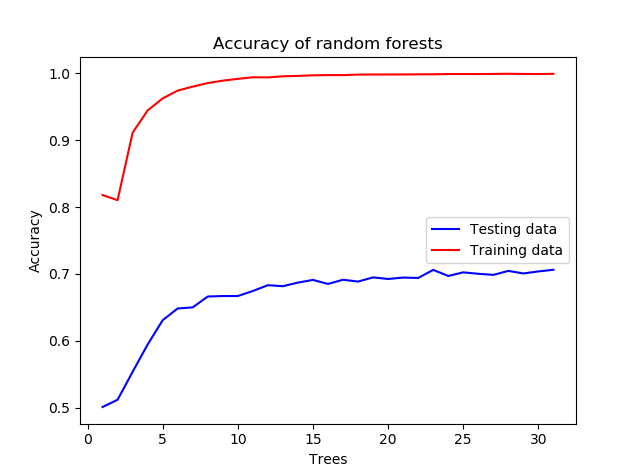
\includegraphics[scale=.7]{images/32treesAcc}\\
So more trees provides a better accuracy. But the classifier starts to have a decent accuracy after 10 trees.

\subsubsection{Difference in number of max\_features}
Here is a plot on how well the accuracy is using different numbers as max\_features:\\
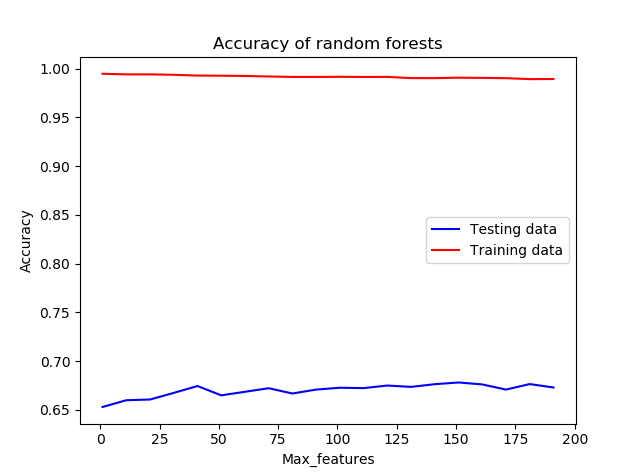
\includegraphics[scale=.7]{images/Max_featuresplot}\\
The number of trees used is 10.\\
\\
The default in the scikitlearn classifier is using the root of the number of all the features as max\_features. Since we have approximately 2000 features, the root becomes 44.72. That's why I computed different accuracies around this number.\\
\\
The plot tells us that it doesn't seem to matter much what we use as max\_features. The optimum in the plot is around 40 which gives us just more reason to stick with the default of using the root of all the features as max\_features.

\subsection{Multilayer perceptrons/Neural Networks}
In this project we use a build in neural network from scikit learn called multilayer perceptrons.
For an explanation of neural networks consult project 2.


\subsection{Voting Classifiers}

Voting classifiers provide a way to combine a collection of classifiers $\varname{clf\_k}$, $k=1,2,\ldots,n$ to form a single classifier, $\varname{voting\_clf}$. 
There are two ways to form voting classifiers, using hard or soft voting. 
In hard voting, to predict the class of a data point $z$, we ask each classifier to predict what class a $z$ belongs to, and then the voting classifier returns the class with the most votes. 
In case of a tie, the scikit learn implementation simply picks the label that comes first when the the labels are sorted. 
For soft voting, we can only use classifiers that assign a probability to each label. 
The voting classifier asks each of $\varname{clf\_k}$ for their probability distribution of the labels, sums them up and picks the label with the highest sum. 

As an example, suppose we have three classifiers $A,B,C$ and $2$-labels. 
Suppose further that on a datapoint $z$ they give the following predictions.

\begin{center}
\begin{tabular}{c|cc}
 & P(-1) & P(1) \\ 
\hline
\hline 
A & 0.55 & 0.45 \\ 
B & 0.51 & 0.49 \\ 
C & 0.10 & 0.90 \\ 
SUM & 1.16 & 1.74
\end{tabular} 
\end{center}

Since both $A$ and $B$ predict the label $-1$, a hard voting scheme will lead to the voting classifier predicting the label $-1$.
On the other hand, if we use a soft voting scheme the voting classifier will predict $1$.
So when using soft voting  we take into account how sure each classifier is in its prediction, but we are restricted to using classifiers that return probabilities.  

\section{Model Selection and Verification}

We used cross validation to decide how to tune our models. 
Because of the size of our data set we felt that three folds would suffice.
To perform the cross validation we used the scikit learn method \funcname{cross\_val\_score}, which returns a list of accuracies, one for each fold. 
We simply took the average of this to the expected accuracy of a method on unseen data, similar to how cross validation for MSE is treated in \cite[Chapter 7.10]{htf:esl}.

\subsection{Single model}

For Logistic Regression, we tune the $C$ parameter. 
The following figure shows the results of our cross validation computations. 

\begin{figure}[H]
\caption{Choosing $C$ for logistic regression.}
\centering
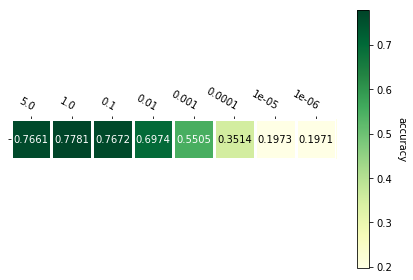
\includegraphics[scale=0.6]{images/logistic_params.png}
\end{figure}

We get the best results when using $C=1$.

For the linear support vector machine the tuning parameter is also called $C$. 
Below are the most important outputs of our cross validation computations. 

\begin{figure}[H]
\caption{Choosing $C$ for support vector machines.}
\centering
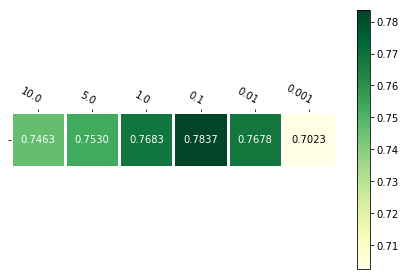
\includegraphics[scale=0.6]{images/linear_svm_params.png}
\end{figure}

Here the best constant is $C = 0.1$.

Random forrest are a voting classifier, so we would expect that more trees yield better results. 
We might be concerned that having too many leafs could lead to over fitting, but as the figure below shows, that is not the case. 
The horizontal axis is the maximal depth of the trees, and the vertical indicates the number of trees. 
 
\begin{figure}[H]
\caption{Tuning random forests.}
\centering
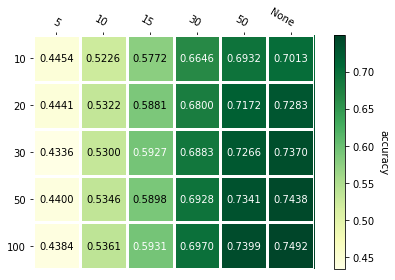
\includegraphics[scale=0.6]{images/forrest_params1.png}
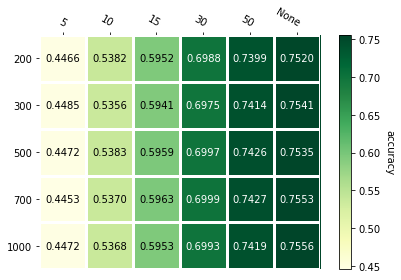
\includegraphics[scale=0.6]{images/forrest_params2.png}
\end{figure}

As expected more trees give better results. 
However, we see that after 100 trees we see a very small increase in accuracy as we add more trees, $0.7492$ for 100 trees vs $0.7556$ for 1000 trees. 
Since the time to train random forests grows with the number of trees, we will restrict our selves to 100 trees when we later turn our attention to voting classifiers. 

The final single model we have used is neural networks, in the form of scikit learns multilayer perceptron classifier. 
Here there are two parameters to tweak, the network structure in the form of number of layers and number of notes in each layer, as well as a regularization parameter called $\alpha$.
The regularization done by $\alpha$ is of the ridge (or $\ell^2$) type that have been discussed in past projects. 
While we tested more settings, the below figures give all the relevant information.

\begin{figure}[H]
\caption{Tuning multilayer perceptron classifier.}
\centering
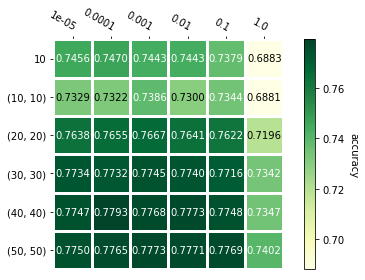
\includegraphics[scale=0.6]{images/mlp_params1.png}
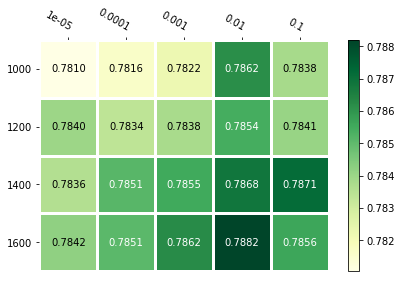
\includegraphics[scale=0.6]{images/mlp_params2.png}
\end{figure}

We see that most setting actually end up in a very similar space.
Increasing the number of nodes does improve the accuracy, but as for the forests, we will for computation reasons restrict ourselves.
This time to the setting of a single layer network with 1000 hidden nodes and $\alpha = 0.01$.

\subsection{Voting Classifiers}

We explored various combinations of the classifiers described above, and bundled them into a single voting classifier. 
Since there is no good way to break ties for a hard voting scheme with only two classifiers voting, we are not investigating them. 
Instead we looked at soft voting for all pairs of classifiers that give probabilities, that is logistic regression, random forests and multilayer preceptrons. 
We also looked at soft voting for all three at once, and two cases of hard voting. 
The results of the cross validation are show in Table \ref{tab:softvoting} (soft voting) and Table \ref{tab:hardvoting} (hard voting). 
Since logistic regression and support vector machines both use a linear approach to classification, and therefore probably give very similar answers, we did not consider triples like svm v forest v logistic with hard voting. 

\begin{table} 
\caption{Soft voting} \label{tab:softvoting}
\begin{center}
\begin{tabular}{lc}
Voting scheme & Average accuracy \\ 
\hline 
\hline
logistic v forest & 0.793308 \\ 
logistic v mlp & 0.785866 \\ 
forest v mlp & 0.798361 \\ 
forest v mlp v logistic &  0.796149 \\ 
\end{tabular} 
\end{center} 
\end{table}
 
\begin{table} 
\caption{Hard voting} \label{tab:hardvoting}
\begin{center}
\begin{tabular}{lc}
Voting scheme & Average accuracy \\ 
\hline 
\hline
svm v forest v mlp &  0.798084 \\ 
svm v forest v mlp v logistic & 0.790843 \\ 
\end{tabular} 
\end{center} 
\end{table}

The first thing we observe is that almost all the voting classifiers are slightly better than the single model classifiers and that they all give very similar accuracies. 
The three highest accuracies are for soft voting with forest v mlp (0.7893), soft voting with forest v mlp v logistic (0.7961), and hard voting with svm v forest v mlp (0.7980).
These are so close, that recommending one over another based only on these number seems very hard.   
Instead we think soft voting with forest v mlp v logistic is likely to be the best option.
This is based on a preference for soft voting over hard voting, and for having more classifiers casting their vote.  

\subsection{Kernels and feature transformation}
 
As we discussed in Section \ref{sssec:kernels}, kernel tricks for support vector machines provide a relative cheap (in memory usage and computation time) way to look at something close to a transformed feature space. 
We used cross validation to test the performance of a polynomial kernel, a sample of our finding are in Figure \ref{fig:polysvm}.

\begin{figure}[H]
\caption{Average accuracies for poly kernel SVM} \label{fig:polysvm}
\centering
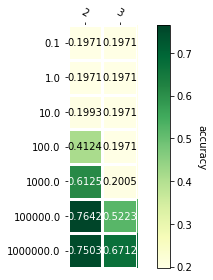
\includegraphics[scale=0.6]{images/svm_poly.png}
\end{figure}

Our take away is that the polynomial kernel does not increase the performance of support vector machines. 
We take this as evidence that using a polynomial transformation of the features is unlikely to improve the other methods. 
Note also that the only interesting polynomial terms would be the interaction terms.
This is because our data points are mainly vectors with entries from $\{0,1\}$.

Another thing to note in Figure \ref{fig:polysvm} is that the average accuracy is the same for $C=0.1, 1, 10$ with a third degree polynomial. 
This might be because those $C$ values end up given the exact same support vectors. 
But by increasing the number of points we allow inside the margin and to cross it, the classifier can depend on more data points and therefore get better accuracy. 
Mostly it is odd though.  

For completeness we also tried the Radial Basis Function kernel, called rbf in scikit learn. 
This uses the kernel function
\[
 K(x_i, x_j) = \exp\left( -\gamma \|x_i - x_j\|^2 \right),
\]
where $\|\cdot\|$ denotes the $2$-norm. 
Again we find that there is no real benefit to using this kernel, even though it is much more computationally demanding than a support vector machine with no kernel.
The results of the cross validation test are show in Figure \ref{fig:rbfsvm}.
The values of $C$ are on the vertical axis, and the values of $\gamma$ on the horizontal axis. 

\begin{figure}[H]
\caption{Average accuracies for rbf kernel SVM} \label{fig:pca_svm}
\centering
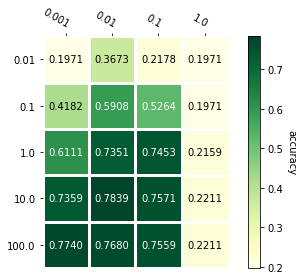
\includegraphics[scale=0.6]{images/svm_rbf.png}
\end{figure}

\subsection{Principal component analysis for support vector machines}

After we had run all the test described above, we realized that we should try to use principal component analysis (PCA) to combine some features. 
The idea being to reduce the number of features while getting features that have a greater explanatory power. 
Figure \ref{fig:pca_svm} shows the results of a 3-fold cross validation of the support vector machine classifier, with no kernel. 
We have varied the number of features the PCA should produce and the regularization parameter $C$. 

\begin{figure}[H]
\caption{Average accuracies for SVM after PCA} \label{fig:rbfsvm}
\centering
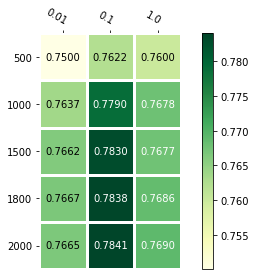
\includegraphics[scale=0.6]{images/pca_svm.png}
\end{figure}

We note that the accuracy increases as the number of components goes up.
However, the accuracy at 2000 is actually slightly ($\approx 0.0004$) higher than the one we got using all the features.
So if we had done this test sooner, using PCA with 2000 features might have been the way to go. 

We only tried the PCA approach for support vector machines. 
This is mostly a time constraint, but given what we have seen about the different classifiers very similar behaviour it does not seem outlandish to suggest that neither of them are likely to improve greatly by using PCA.

\section{Results and discussion} \label{sec:results}

As mentioned in the introduction our data set comes from a kaggle competition. 
The competition is over, but allows late submissions, so submitted our best classifier using the script one can see at \url{https://github.com/jonabaa/Project3/blob/master/code/Kaggle%20submission%20script.ipynb}. 
The results are not public, so below is a screen shot of our result.

\begin{figure}[H]
\caption{Kaggle result} \label{fig:kaggleresult}
\centering
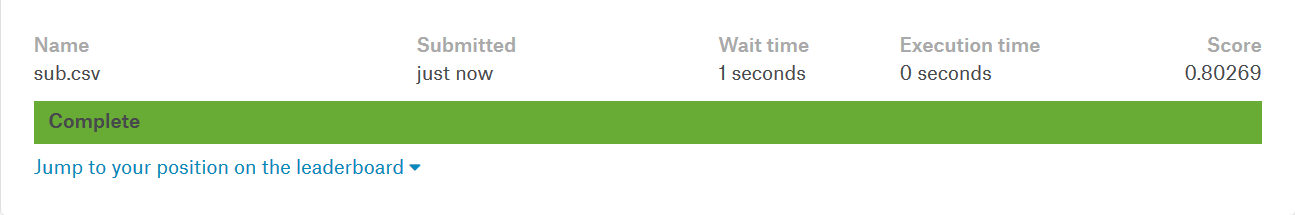
\includegraphics[scale=0.3]{images/kaggle_result.png}
\end{figure}

We got an accuracy of 0.80269. 
Which would have given us a somewhat unimpressive 231st place in the competition. 
It is worth noting the the highest accuracy achieved in the competition is 0.82783, so we are only off by about 2\% worth of accuracy.

There are some things we could have done to do better in the competition:
We could base our \funcname{CountVectorizer} on the test set, so we only consider ingredients that we will be tested on as features. 
Since there is no submission limit, we could also just have submitted various attempt and seen which one got a better score.
But these are competition solutions. 

It is also possible that we should have included the \varname{min\_df} parameter in our search for the best parameters for each method. 
This would correspond to finding an optimal matrix representation of the raw recipe data.  
In general we might have spent more time exploring the quality of the data. 
There are for instance 22 recipes that only have one ingredient, including a French and an Indian recipe both calling only for butter. 
There is also an Indian recipe calling only for ``grained,'' which must almost surely be a typo of sorts. 
However, we did not see a great systematic way to improve the quality of our data, and there were way to many recipes to go through by hand. 

We might also have taken a more linguistic approach and looked for key words in recipes. 
If you are specifically asked to use Italian sausages, chances seem very good that you are making Italian food. 
We assume that there are other similar but less obvious ways one could classify some recipes.
Then once these easy ones were out of the way, we could turn to machine learning techniques, but we did not explore this avenue.     

To get an understanding on where our classifier fails, we split or training data into 2, trained on one part and then tried to to predict the other.
Figure \ref{fig:confusion} shows the confusion matrix for this test.
Each row is normalized, so that the row labeled Italian shows that of the Italian recipes 0.85 were correctly classified as Italian, but 0.04 were classified as French. 
We also see that French is in fact the most common misclassification for Italian recipes. 

\begin{figure}
\caption{Confusion matrix} \label{fig:confusion}
\centering
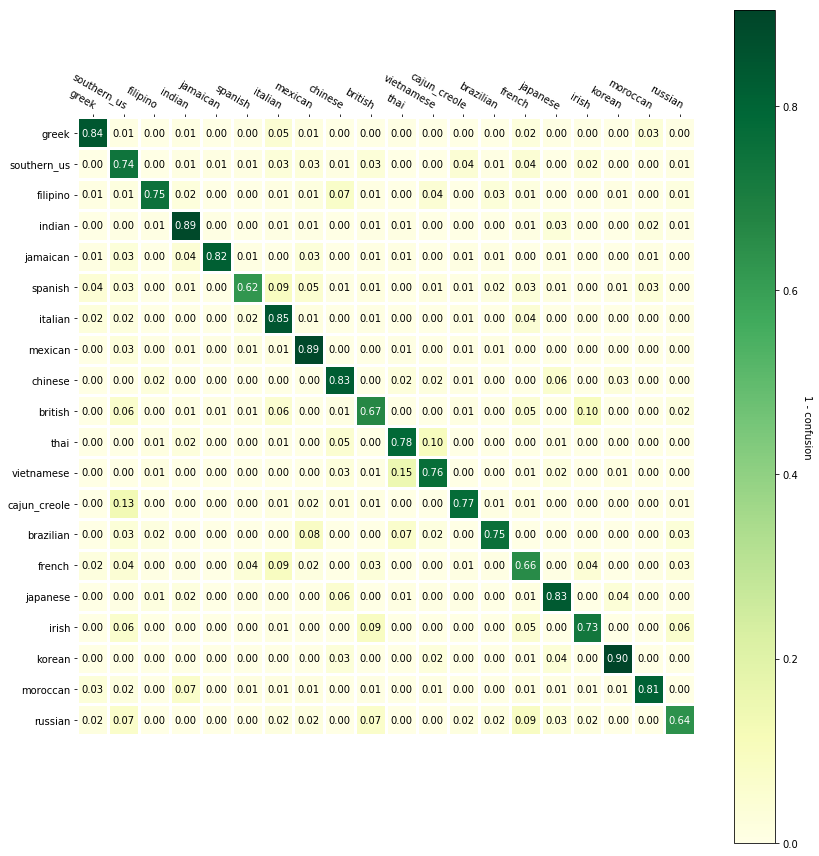
\includegraphics[scale=0.6]{images/confusion.png}
\end{figure}

The confusion matrix shows that the relative biggest misclassification is for Cajun Creole food, where 13\% is incorrectly label southern US. 
As Cajun Creole stems from Louisianan, which is very much in the southern US, this does not seem like a big mistake. 
In fact, we see the confusion matrix as showing that our classifier does a mostly good job.
It might not always be right, but when it is wrong it is not very wrong, as it might confuse cuisines that are intuitively close like Irish and British. 
 
\section{Conclusion} \label{sec:conclusion}

We saw that almost all our single classifiers did a fine job.
The best tuned versions have predicted accuracies of $\approx 0.78$ for logistic regression, support vector machines, and multilayer perceptrons, and $\approx 0.75$ for random forest.
Using voting classifiers we could get the predicted accuracy upto $\approx 0.79$. 
In the kaggle competition, where we got an accuracy of $\approx 0.80$ the winner got $\approx 0.82$.

The results suggest that the data splits into a large chunk that is very easy to classify, and a smaller chunk where classification is very hard.
On this smaller chunk winning even a single percentage point of extra accuracy requires cleverness. 
%%%%%%%%%%%%%%
%Bibliography
\bibliographystyle{apalike}
\bibliography{refs}	% expects file "refs.bib"
%%%%%%%%%%%%%%


\end{document}
